\documentclass[a4paper,12pt]{article} % тип документа

% report, book

% Рисунки
\usepackage{graphicx}
\usepackage{wrapfig}

\usepackage{hyperref}
\usepackage[rgb]{xcolor}
\hypersetup{				% Гиперссылки
    colorlinks=true,       	% false: ссылки в рамках
	urlcolor=blue          % на URL
}

%  Русский язык

\usepackage[T2A]{fontenc}			% кодировка
\usepackage[utf8]{inputenc}			% кодировка исходного текста
\usepackage[english,russian]{babel}	% локализация и переносы


% Математика
\usepackage{amsmath,amsfonts,amssymb,amsthm,mathtools} 


\usepackage{wasysym}

\author{Анна Назарчук Б02-109}
\title{1.4.5 Исследование колебаний струны}
\date{}
\begin{document}
\maketitle
\section{Теоретические сведения}
Струна - однородная гибкая упругая нить (например, струна гитары). В натянутой струне возникает поперечная упругость, то есть способность сопротивляться любому изменению формы без изменения объема. 

Рассомтрим уравнение волны на струне, сила натяжения существенно превышает вес струны для отсутствия провисаний. $tg\alpha = \frac{\partial y}{\partial x}$ - угол наклона касательной к графику. Для вертикального движения элемента струны:
\begin{equation}
\delta m \frac{\partial ^ 2 y}{\partial t^2} = -T_1\sin \alpha_1 + T_2\sin \alpha_2
\end{equation}

\begin{figure}[h!]
\begin{center}
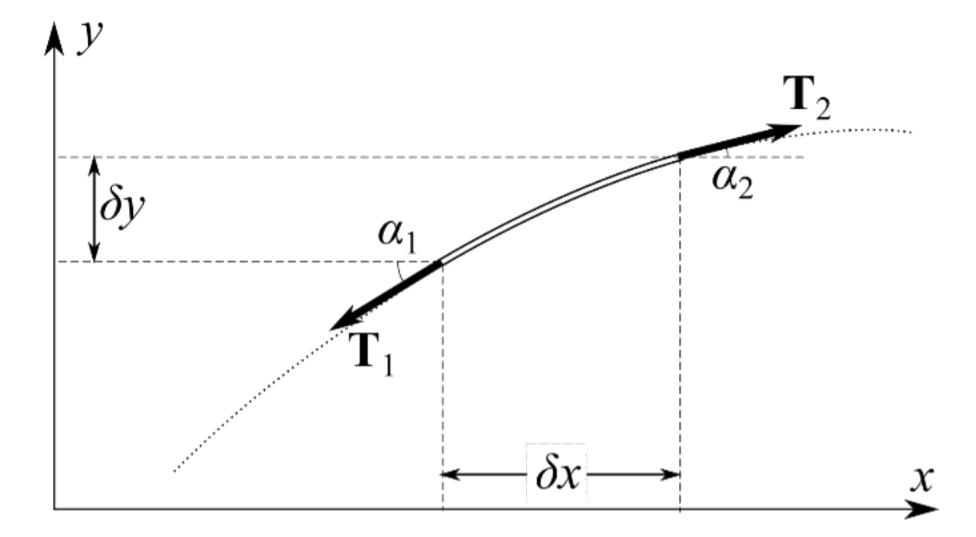
\includegraphics[width=1\textwidth]{Вывод}
\end{center}
\caption{Вывод уравнения волны в струне} \label{вывод}
\end{figure}

Длина участка струны в смещенном состоянии почти равна длине участка в положении равновесия, поэтому: $T_1\approx T_2\approx T$. Углы наклона малы, откуда:
\begin{equation}
\rho_l \frac{\partial ^ 2 y}{\partial t^2} = \frac{-T_1\sin \alpha_1 + T_2\sin \alpha_2}{\partial x} \approx T \frac{\alpha_2-\alpha_1}{\partial x}\to T \frac{\partial \alpha}{\partial x}
\end{equation}
$\rho_l = m/l$ -погонная плотность струны. Пусть $u = \sqrt{t/\rho_l}$
Тогда уравнение свободных малых поперечных колебаний
струны:
\begin{equation}
\frac{\partial ^ 2 y}{\partial t^2} = u^2\frac{\partial ^ 2 y}{\partial x^2}
\end{equation}


\subsection{Измерения и обработка данных}

\begin{table} \label{} \caption{} \begin{tabular}{|c|c|c|c|c|c|c|} \hline m, г & $\rho$, мг/м & n & L, см & nu, Гц & u, м/$c^2$ & $\sigma_u$, м/$c^2$ \\ \hline 1096.3 & 568.4 & 1 & 50.3 & 141.16 & 140.915 & 0.568 \\ \hline 1096.3 & 568.4 & 3 & 50.3 & 414.4 & 140.915 & 0.568 \\ \hline 1096.3 & 568.4 & 5 & 50.3 & 695.9 & 140.915 & 0.568 \\ \hline 1096.3 & 568.4 & 7 & 50.3 & 965.9 & 140.915 & 0.568 \\ \hline 1096.3 & 568.4 & 9 & 50.3 & 1272.12 & 140.915 & 0.568 \\ \hline 1096.3 & 568.4 & 2 & 50.3 & 283.26 & 140.915 & 0.568 \\ \hline 1096.3 & 568.4 & 4 & 50.3 & 568.16 & 140.915 & 0.568 \\ \hline 1096.3 & 568.4 & 0.5 & 50.3 & 70.82 & 140.915 & 0.568 \\ \hline 1578.7 & 568.4 & 1 & 50.3 & 161.49 & 165.356 & 0.343 \\ \hline 1578.7 & 568.4 & 3 & 50.3 & 491.54 & 165.356 & 0.343 \\ \hline 1578.7 & 568.4 & 5 & 50.3 & 824.02 & 165.356 & 0.343 \\ \hline 1578.7 & 568.4 & 2 & 50.3 & 327.1 & 165.356 & 0.343 \\ \hline 602.3 & 568.4 & 2 & 50.3 & 200.54 & 102.549 & 0.288 \\ \hline 602.3 & 568.4 & 1 & 50.3 & 102.41 & 102.549 & 0.288 \\ \hline 602.3 & 568.4 & 3 & 50.3 & 306.81 & 102.549 & 0.288 \\ \hline 602.3 & 568.4 & 5 & 50.3 & 510.33 & 102.549 & 0.288 \\ \hline 940.3 & 568.4 & 1 & 50.3 & 128.2 & 129.866 & 0.264 \\ \hline 940.3 & 568.4 & 3 & 50.3 & 384.76 & 129.866 & 0.264 \\ \hline 940.3 & 568.4 & 5 & 50.3 & 647.31 & 129.866 & 0.264 \\ \hline 940.3 & 568.4 & 2 & 50.3 & 257.77 & 129.866 & 0.264 \\ \hline 1427.7 & 568.4 & 1 & 50.3 & 158.36 & 160.171 & 0.111 \\ \hline 1427.7 & 568.4 & 3 & 50.3 & 476.9 & 160.171 & 0.111 \\ \hline 1427.7 & 568.4 & 5 & 50.3 & 796.81 & 160.171 & 0.111 \\ \hline 1427.7 & 568.4 & 2 & 50.3 & 318.16 & 160.171 & 0.111 \\ \hline \end{tabular} \end{table}
\begin{equation}
\rho_l = (552.64 \pm 3.59) \cdot  10^{-6} \text{кг/м}
\end{equation}
\begin{figure}[h!]
\begin{center}
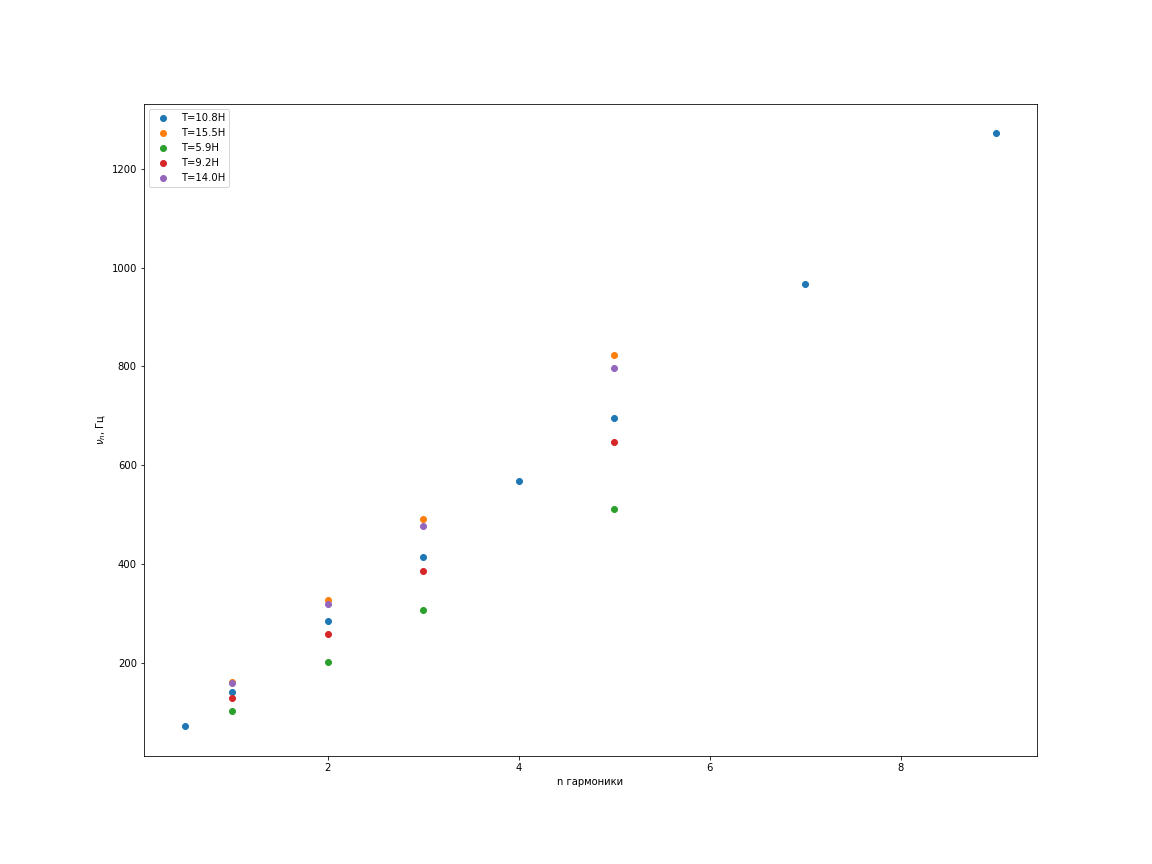
\includegraphics[width=\textwidth]{nu от n}
\end{center}
\caption{Зависимость $\nu$ от $n$} \label{график}
\end{figure}

\begin{figure}[h!]
\begin{center}
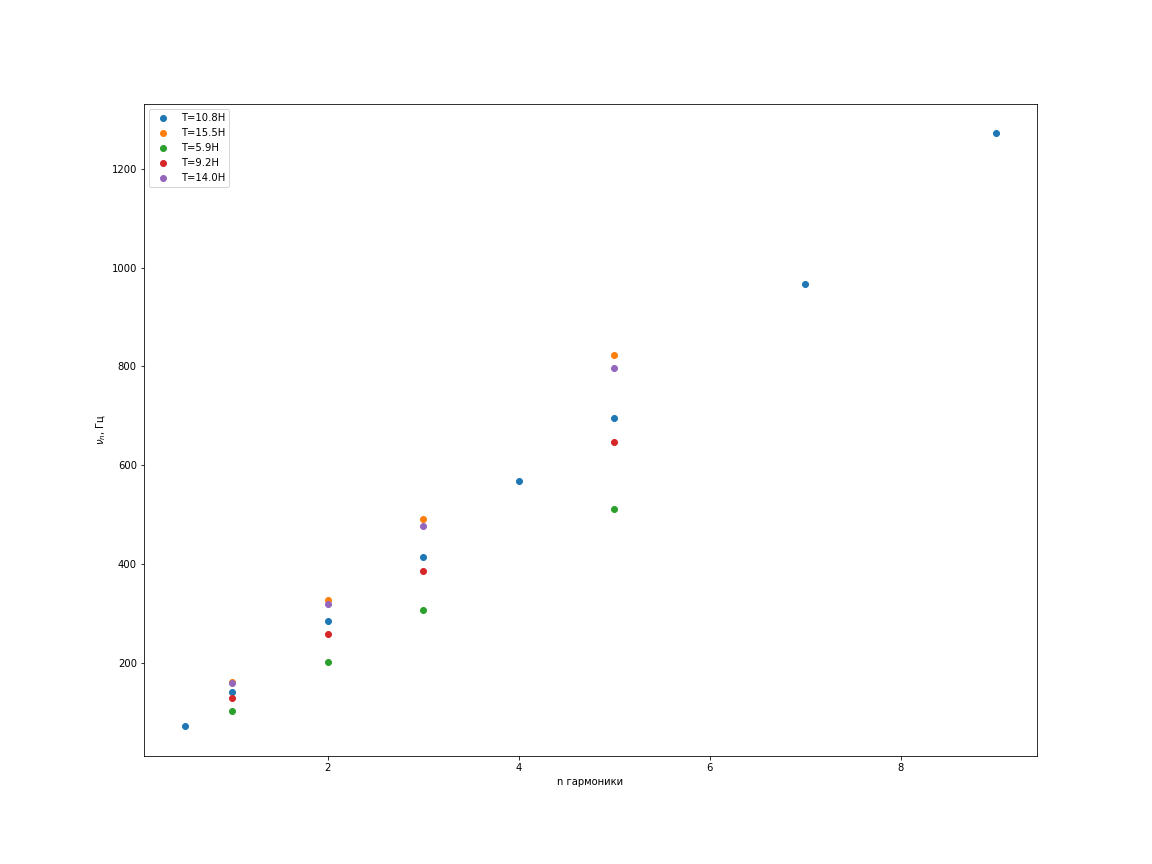
\includegraphics[width=\textwidth]{u^2 от T }
\end{center}
\caption{Зависимость $u^2$ от $T$} \label{график}
\end{figure}
\begin{equation}
Q = \frac{\nu_\text{рез}}{\bigtriangleup \nu} = 1.7 \cdot 10^{-3}
\end{equation}
\end{document}